\documentclass{llncs}
\usepackage{graphicx}
\usepackage{color}
\usepackage[english]{babel}
\usepackage[utf8]{inputenc}
\usepackage{pgfplots}
\usepackage{algpseudocode}
\usepackage{algorithm}
\usetikzlibrary{patterns}
\begin{document}

\title{Trust in information sources on a competitive and distributed environment}
\author{João Pedro Dias, João Correia and Eduardo Martins}
\institute{Faculdade de Engenharia da Universidade do Porto, Portugal\\\email{\{ei11137,ei12159,ei11104\}@fe.up.pt}}

\maketitle

\begin{abstract}

Distributed systems based on agents are sometimes used in competitive environments with information sources that we have little or none knowledge about. In these cases we need to make the agents take the best decisions on what information source is most valuable to them. For this we have little more than the agent experience itself. This paper simulates this type of environment approaching a question and answer game, where the agents have to decide the best information source for each question based on question thematic. For this experiment we use a set of computation trust algorithms for making decisions on the best information sources for each question, and we verified that the most simple approaches are capable of good results when the information sources maintain the same behaviour throughout the execution. Complex approaches can get us better results when the informations sources behaviour changes.

\keywords{Artificial Intelligence, Multi-Agent, Computational Trust, Distributed Systems}
\end{abstract}

\section{Introduction}\label{sec:Introduction}

Multi-agent distributed systems are in use in a lot of cases from smart-grids\cite{intro} to autonomous on-line auctions\cite{introtwo}. There are some cases when the agents in this systems need to take actions based in information sources which the agents don't know about. And, additionally, there are cases where this agents are competing between themselves. In these cases there is a need to use computation trust algorithms capable of choosing and using the most valuable information sources for each type of information we needed and get better results over other agents.

The purpose of this work is to examine the efficiency of different trust algorithms against a similar environment.The specific goals are:
\begin{itemize}
\item To demonstrate that trust algorithms are more suited for this type of environment.
\item To demonstrate a possible architecture for this kind of systems.
\item To ensure all the communication between agents.
\end{itemize}

In this paper we start presenting the chosen scenario at section \ref{Scenario description}, followed by identification of the agents in the systems and algorithms used in section \ref{sec:Specification}. Next we show in section \ref{sec:Development} the used tools and the interaction protocol. Finally we present all the experiments realized at section \ref{sec:Experiments} and a conclusion in section \ref{sec:Conclusion}.

\subsection{Scenario description}\label{Scenario description}

The competitive environment is easily replicated and modelled as a game of questions and answers, where every player is an agent and there is a list of information sources with one master agent responsible for validating the answers by the players.

With the purpose of adding variety to the information sources, there are questions distributed between 5 thematics: Sports, History, Science, Arts and Places. The information sources can have specific knowledge in one theme or more as well they can be totally random.

The game sequence begins with the master doing a random question to all players with four answer options. Then all the players in-game choose one and only one information source that they will use to answer that question. The choice of the information source correctly is the core function of the players, since the player answers depending on that. This choice depends on the trust algorithm used by the player and by the category of the question. The game ends when the master reaches the number of questions defined to be done.

\section{Specification}\label{sec:Specification}

\subsection{Agents identification and specification}\label{sec:Agents}

With the purpose to have the most precise simulation of the environment described, there was the need to implement different types of agent behaviours that can represent every role in the system, namely, a master, various players and various information sources, each one with a different role as identified in Table \ref{Agent}. 

\begin{table}
\begin{tabular}{| p{1.3cm}| p{3.2cm}| p{3cm}| p{4.3cm}|}
\hline
\textbf{Agent} & \textbf{Input} & \textbf{Output} & \textbf{Specification}                                                                                                                                                                                                                                  \\\hline
\textit{Master} & Number of iterations and Questions/Answers Database                                                           & Execution statistics (number of right/wrong questions by player) & Game engine, responsible for making questions and validating answers. \\ \hline
\textit{Player} & Theme, Question, 4 answer options & Answer to the question. & Ask one of the \textit{experts} for the answer. This choice depends on the trust algorithm implemented on the player.\\ \hline
\textit{Expert} & Question. & Answer for the given question. & Answer the question made even if its not in the knowledge domain of the expert. If the question its outside the knowledge domain it will give a random answer. \\\hline
\end{tabular}\\
\caption{Different agents tasks.}
\label{Agent}
\end{table}

Specifying each one of the agents present in the system, we have four players: 
\begin{itemize}
\item Player \textit{RANDOM}: A player with no trust algorithm implemented which chooses one expert to answer randomly. 
\item Player \textit{DUMMY}: A player which uses a very simple algorithm that build a matrix based on trust (experts/theme). Specified in section \ref{Trust}.
\item Player \textit{FIRE}: The player uses the \textit{FIRE} algorithm \cite{Fire}. Specified in section \ref{Trust}.
\item Player \textit{BETA}: The player uses the \textit{BETA} algorithm \cite{Beta}. Specified in section \ref{Trust}.
\end{itemize}
and nine experts as information sources:
\begin{itemize}
\item \textit{Sports} Expert: Have 100\% expertise in questions about Sports.
\item \textit{History} Expert: Have 100\% expertise in questions about History.
\item \textit{Science} Expert: Have 100\% expertise in questions about Science.
\item \textit{Places} Expert: Have 100\% expertise in questions about Places.
\item \textit{Arts} Expert: Have 100\% expertise in questions about Arts.
\item \textit{All} Expert: Have 100\% expertise in all thematics.
\item \textit{Random} Expert: Have a 25\% probability of answer correctly (the number of possible answer is 4).
\item \textit{Variable} Expert: Have a change to get right all the first 50 questions or less.
\item \textit{Common} Expert: Have 50\% knowledge over each thematic.
\end{itemize}

\subsection{Trust algorithms}\label{Trust}

The various players in game have different behaviour accordantly with the trust algorithm they use. As listed we have three trust algorithms implemented. This algorithms in major part are only experience based due to the competitive environment.

The \textit{DUMMY} player who uses a basic approach of building a matrix given points for each information source depending on its performance on each theme, in this case specifically, we give one positive point for each right answer and one negative for each wrong answer. In each iteration the player will use the experts with the biggest punctuation for that question theme. This algorithm implementation is described on Algorithm \ref{alg:dummy}.


\begin{algorithm}
\begin{algorithmic}[1]
  \Function{Pontuation}{$A[cat][exp]$, $answer$, $cat$, $exp$}
 	\If{$answer == true$}
    \State {$A[cat][exp] \leftarrow A[cat][exp]++$ };
 	\Else
    \State {$A[cat][exp] \leftarrow A[cat][exp]--$ };
    \EndIf
  \EndFunction
  \Function{GetBestExpertByCategory}{$A[cat][exp]$, $cat$}
  	\State {$tempPoints \leftarrow -\infty$};
  	\State {$tempExpert \leftarrow NULL$};
	\For {$i \leftarrow 1, size(A[category])$}
		\If {$A[i] == cat$}
		\For {$j \leftarrow 1, size(A[i][expert])$}
			\If {$A[i][expert]>temp$}
			\State {$tempPoints \leftarrow A[i][expert]$};
			\State {$tempExpert \leftarrow expert$};
			\EndIf
    	\EndFor
    	\EndIf
    \EndFor
    \Return {$tempExpert$};
  \EndFunction
\end{algorithmic}
\caption{DUMMY Algorithm}\label{alg:dummy}
\end{algorithm}

The \textit{BETA} player who uses the BETA reputation system \cite{Beta} for choosing the best information source for each question. This algorithm uses, as said in \textit{The beta reputation system}, the \textit{"beta probability density functions to combine feedback and derive reputation ratings"}\cite{Beta}.

The \textit{FIRE} player who uses an approximation to the FIRE algorithm \cite{Fire} to choose the expert to use. This algorithm uses its experience, but uses as well opinions from other agents, dividing itself in four different parts, two directed to experience and two directed to opinions. For this specific case this algorithm can be a bad choice since it's a competitive environment and the communication between concurrent agents can be non-existent. So, in our specification, this player will have a collaborator that acts like another normal player with experience-based behaviour, but with the difference that it will give an opinion to the \textit{FIRE} player with the ratio of wrong/right questions for each expert existent in game.

\subsection{System architecture}\label{sec:Architecture}
The system architecture follows accordantly with the framework used (described in section \ref{sec:Tools}), ensuring all the synchronous communication needs between agents for the correct simulation and evaluation. In this architecture as showed in Fig.\ref{arch} we have one and only one master agent, a minimum of one player and a minimum of one information source. 

\begin{figure}
	\centering
    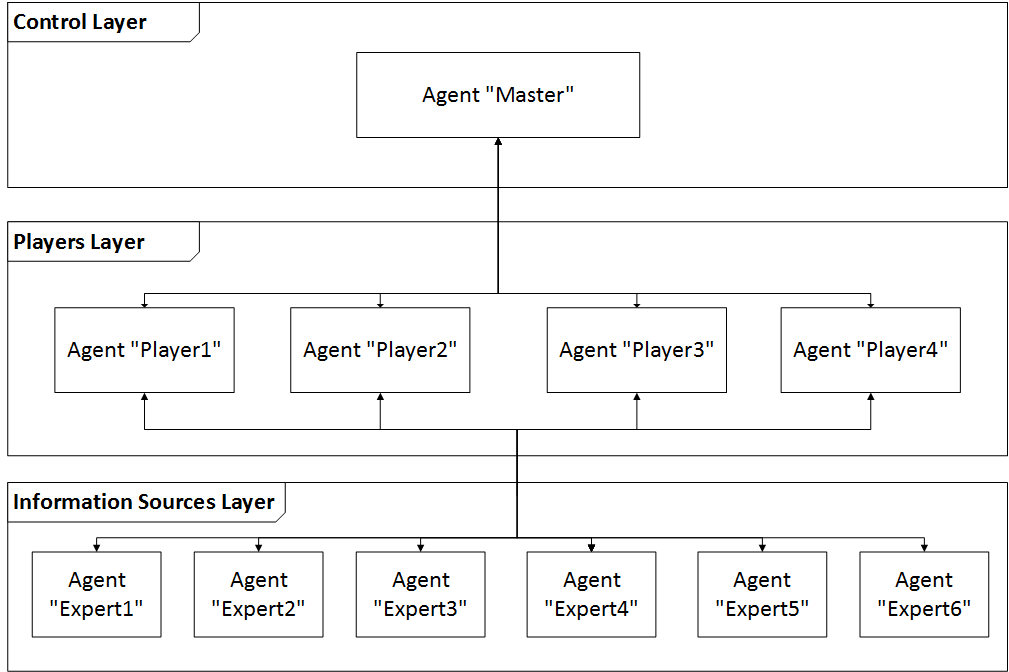
\includegraphics[width=0.8\textwidth]{arch.png}
    \caption{System architecture. The number of agents \textit{player} and \textit{expert} can vary.}
    \label{arch}
\end{figure}


\section{Development}\label{sec:Development}
\subsection{Tools}\label{sec:Tools}

For implementing the system its used the JADE\footnote{JAVA Agent DEvelopment Framework is an open source platform for peer-to-peer agent based applications.} framework, that is fully implemented in the JAVA programming language, and so it is cross-platform. It simplifies the implementation of this kind of system through a middle-ware that complies with the FIPA\footnote{ Foundation for Intelligent Physical Agents is a body for developing and setting standards for heterogeneous and interacting agents and agent-based systems.} specifications for multi-agent systems \cite{architecture}.

\begin{figure}
	\centering
    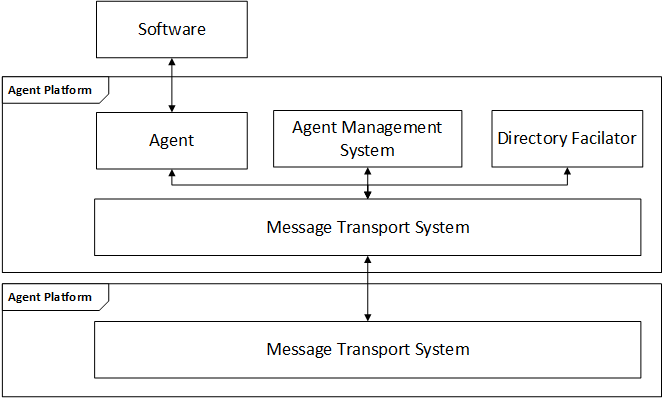
\includegraphics[width=0.8\textwidth]{fipa.png}
    \caption{Agent Management Reference Model}
    \label{jade}
\end{figure}

This middle-ware consists in various components based on FIPA standard architecture (Fig.\ref{jade}):
\begin{itemize}
\item The Agent Management System (AMS) controls the platform. Is the only one who can create and destroy other agents, destroy containers and stop the platform. Also, it contains a list of Agent Identifiers (AID) with every agent on the system.
\item The Directory Facilitator (DF) provides a directory which announces which agents are available on the platform.
\item The Message Transport Service (MTS) is the default method of communication between agents. Each message its compliant with the FIPA Agent Communication Language (ACL).
\end{itemize}

\subsection{Interaction protocol}\label{sec:Interaction}

Due to the JADE being message compliant to the "FIPA ACL Message Structure Specification" give us the capacity of label all the communication between agents with FIPA performatives \cite{msg}.

With this, it was established a interaction protocol between the agents in the system as showed in Fig.\ref{sequence}. The execution start with the master asking a question and it enters in a loop of question followed by a answer by the player and a validation of the answer by the master. It ends when the master reach the pre-defined number of questions to make.

\begin{figure}
	\centering
    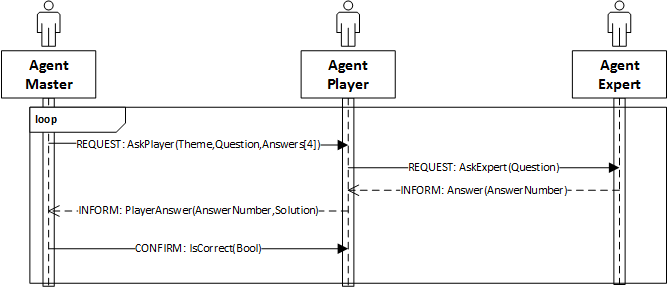
\includegraphics[width=1\textwidth]{sequence.png}
    \caption{System's sequence diagram.}
    \label{sequence}
\end{figure}


\section{Experiments \& Discussion}\label{sec:Experiments}

To test the system developed it was carried out some experiences, with the various agents developed and presented in section \ref{sec:Agents}, analysing the different results obtained. All tests are made using the same question database that contains five question per thematic. Additionally its used a fixed number of questions, in the case, 200 questions.

To certify that all communication are been done correctly it was made various experiences with one single expert with 100\% knowledge in all thematics.

The experiments carried give us a perspective of the behaviour of the different algorithms used as showed in section \ref{Trust}. So for a better capacity of presenting more precise conclusions we made a set of experiments with different groups of experts.

Between all the experiments done, the results of the different players changes during the different tries for each experiment, more specifically:
\begin{itemize}
\item \textit{FIRE} player varies in the maximum of 21 answers;
\item \textit{DUMMY} player varies in the maximum of 16 answers;
\item \textit{RANDOM} player varies in the maximum of 18 answers;
\item \textit{BETA} player varies in the maximum of 11 answers;

\end{itemize}

\begin{figure}
\centering
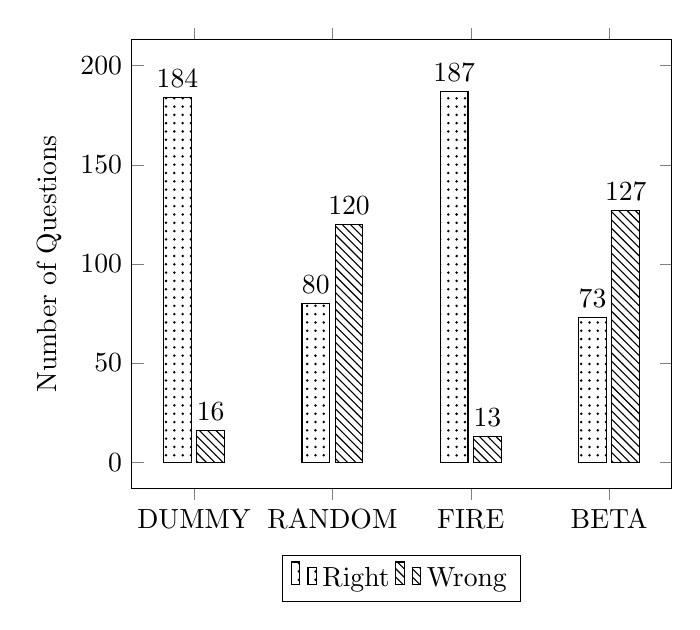
\begin{tikzpicture}
\begin{axis}[
    ybar,
    enlargelimits=0.15,
    legend style={at={(0.5,-0.15)},
      anchor=north,legend columns=-1},
    ylabel={Number of Questions},
    symbolic x coords={DUMMY,RANDOM,FIRE,BETA},
    xtick=data,
    nodes near coords,
    nodes near coords align={vertical},
    ]
\addplot [pattern = dots] coordinates {(DUMMY,184) (RANDOM,80) (FIRE,187) (BETA,73)};
\addplot [pattern = north west lines] coordinates {(DUMMY,16) (RANDOM,120) (FIRE,13) (BETA,127)};
\legend{Right,Wrong}
\end{axis}
\end{tikzpicture}
\caption{Experience with five experts with 100\% knowledge by question theme.}
\label{allexperts}
\end{figure}

In the first experiment, Experiment \ref{allexperts}, we used one expert per thematic, each one with 100\% knowledge in each theme. This is our first experiment used to analyse the behaviour of the different players in a environment were the information by thematic is distributed among different sources. The results pointed out by the experiment showed us that the algorithms that use classification of experts by thematic, like FIRE or DUMMY, given us better results than the algorithms that just analyse the number of questions answered right or wrong by expert like the BETA algorithm.

\begin{figure}
\centering
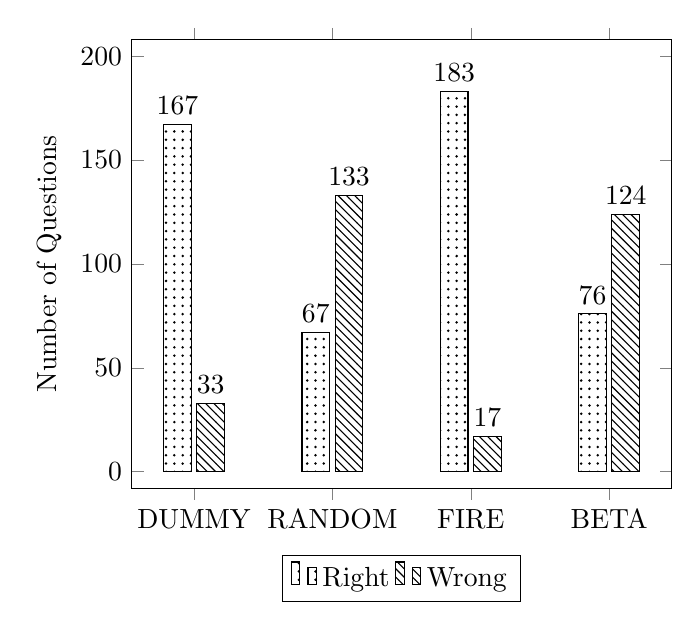
\begin{tikzpicture}
\begin{axis}[
    ybar,
    enlargelimits=0.15,
    legend style={at={(0.5,-0.15)},
      anchor=north,legend columns=-1},
    ylabel={Number of Questions},
    symbolic x coords={DUMMY,RANDOM,FIRE,BETA},
    xtick=data,
    nodes near coords,
    nodes near coords align={vertical},
    ]
\addplot [pattern = dots] coordinates {(DUMMY,167) (RANDOM,67) (FIRE,183) (BETA,76)};
\addplot [pattern = north west lines] coordinates {(DUMMY,33) (RANDOM,133) (FIRE,17) (BETA,124)};
\legend{Right,Wrong}
\end{axis}
\end{tikzpicture}
\caption{Experience with five experts with 100\% knowledge by question theme and one random expert.}
\label{allexpertsrandom}
\end{figure}

The Experiment \ref{allexpertsrandom} showed us that even when we add a random expert to the Experiment \ref{allexperts}, the results given by the player have small changes only.

\begin{figure}
\centering
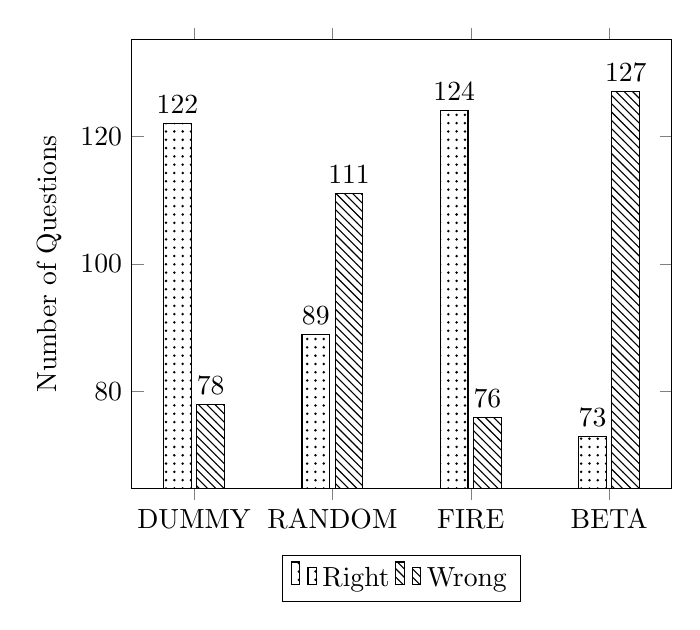
\begin{tikzpicture}
\begin{axis}[
    ybar,
    enlargelimits=0.15,
    legend style={at={(0.5,-0.15)},
      anchor=north,legend columns=-1},
    ylabel={Number of Questions},
    symbolic x coords={DUMMY,RANDOM,FIRE,BETA},
    xtick=data,
    nodes near coords,
    nodes near coords align={vertical},
    ]
\addplot [pattern = dots] coordinates {(DUMMY,122) (RANDOM,89) (FIRE,124) (BETA,73)};
\addplot [pattern = north west lines] coordinates {(DUMMY,78) (RANDOM,111) (FIRE,76) (BETA,127)};
\legend{Right,Wrong}
\end{axis}
\end{tikzpicture}
\caption{Experience with two experts with 100\% knowledge in the thematics Places and History}
\label{twoexperts}
\end{figure}

In the Experiment \ref{twoexperts} we verified how that the lack of knowledge is manage by the different players. The results showed us that the percentage of right answers decreases due to this lack of knowledge, since the players are limited too the only two players that exists in the environment.

\begin{figure}
\centering
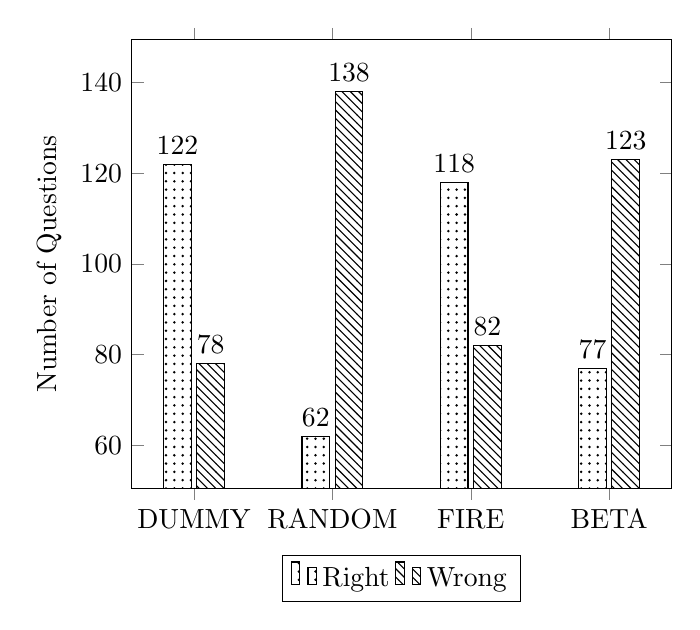
\begin{tikzpicture}
\begin{axis}[
    ybar,
    enlargelimits=0.15,
    legend style={at={(0.5,-0.15)},
      anchor=north,legend columns=-1},
    ylabel={Number of Questions},
    symbolic x coords={DUMMY,RANDOM,FIRE,BETA},
    xtick=data,
    nodes near coords,
    nodes near coords align={vertical},
    ]
\addplot [pattern = dots] coordinates {(DUMMY,122) (RANDOM,62) (FIRE,118) (BETA,77)};
\addplot [pattern = north west lines] coordinates {(DUMMY,78) (RANDOM,138) (FIRE,82) (BETA,123)};
\legend{Right,Wrong}
\end{axis}
\end{tikzpicture}
\caption{Experience with two experts with 100\% knowledge in the thematics Places and History, plus a random expert.}
\label{twoexpertsrandom}
\end{figure}

The Experiment \ref{twoexpertsrandom} we verified how that the lack of knowledge is manage by the different players in a environment where exists a random information source. The results showed us that the percentage of right answers decreases as showed in experiment \ref{twoexperts} and the addition of the random expert don't affect significantly the results.

\begin{figure}
\centering
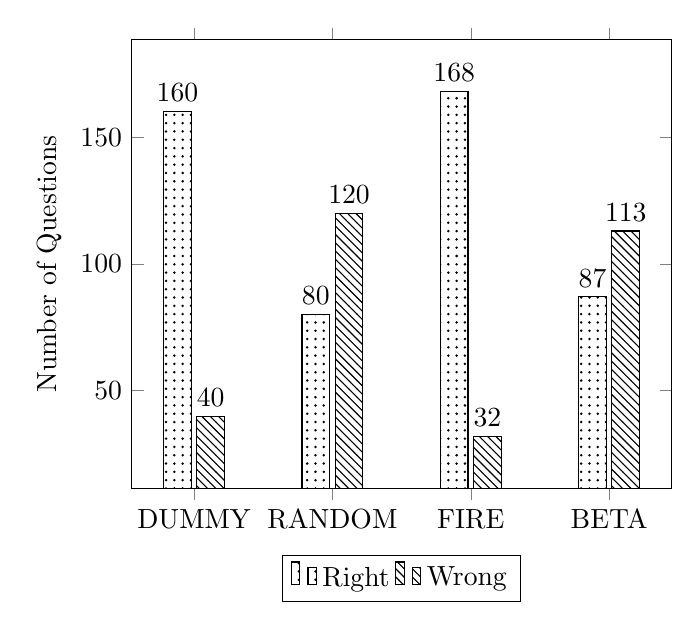
\begin{tikzpicture}
\begin{axis}[
    ybar,
    enlargelimits=0.15,
    legend style={at={(0.5,-0.15)},
      anchor=north,legend columns=-1},
    ylabel={Number of Questions},
    symbolic x coords={DUMMY,RANDOM,FIRE,BETA},
    xtick=data,
    nodes near coords,
    nodes near coords align={vertical},
    ]
\addplot [pattern = dots] coordinates {(DUMMY,160) (RANDOM,80) (FIRE,168) (BETA,87)};
\addplot [pattern = north west lines] coordinates {(DUMMY,40) (RANDOM,120) (FIRE,32) (BETA,113)};
\legend{Right,Wrong}
\end{axis}
\end{tikzpicture}
\caption{Experience with five experts with 100\% knowledge in each thematic and the \textit{Variable} expert}
\label{vary}
\end{figure}

At the Experiment \ref{vary} we add the \textit{Variable} expert.  This experiment give us a perspective of the way that the different algorithms used adapt to the addition of a variable information source. Namely, this showed that the \textit{FIRE} and \textit{DUMMY} algorithms are more slow to adapt to this changes and, on the other hand, the \textit{BETA} adapts more quickly to this change.

\begin{figure}
\centering
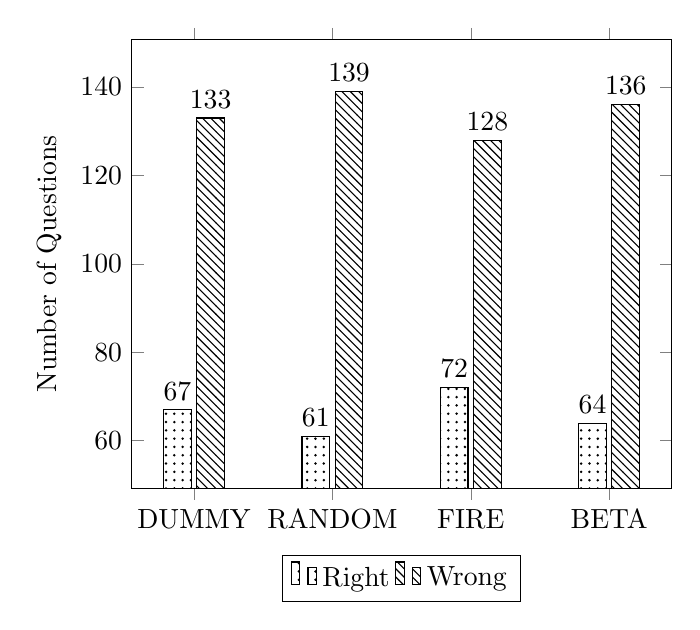
\begin{tikzpicture}
\begin{axis}[
    ybar,
    enlargelimits=0.15,
    legend style={at={(0.5,-0.15)},
      anchor=north,legend columns=-1},
    ylabel={Number of Questions},
    symbolic x coords={DUMMY,RANDOM,FIRE,BETA},
    xtick=data,
    nodes near coords,
    nodes near coords align={vertical},
    ]
\addplot [pattern = dots] coordinates {(DUMMY,67) (RANDOM,61) (FIRE,72) (BETA,64)};
\addplot [pattern = north west lines] coordinates {(DUMMY,133) (RANDOM,139) (FIRE,128) (BETA,136)};
\legend{Right,Wrong}
\end{axis}
\end{tikzpicture}
\caption{Experience with the \textit{Variable} expert and the \textit{Common} expert.}
\label{varycommon}
\end{figure}

The Experiment \ref{varycommon} adds to the environment the \textit{Variable} and the \textit{Common} experts only. This showed us how the different players manage the existence of one information source with only a percentage of knowledge(\textit{Common}) and one with variable knowledge in the execution runtime. At the end of the experiment we verified that the \textit{BETA} adapts well to this environment given similar results to the other experiments and the other players suffer more in this environment given worst results than in the other experiments.
 
\begin{figure}
\centering
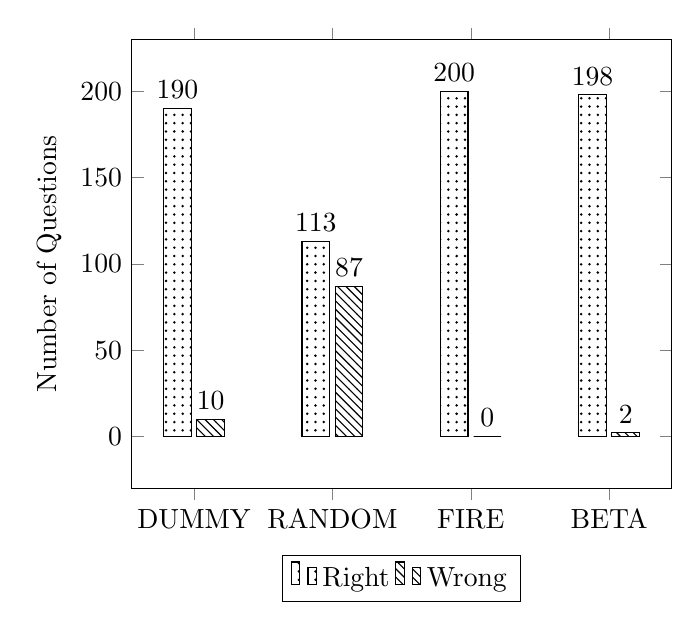
\begin{tikzpicture}
\begin{axis}[
    ybar,
    enlargelimits=0.15,
    legend style={at={(0.5,-0.15)},
      anchor=north,legend columns=-1},
    ylabel={Number of Questions},
    symbolic x coords={DUMMY,RANDOM,FIRE,BETA},
    xtick=data,
    nodes near coords,
    nodes near coords align={vertical},
    ]
\addplot [pattern = dots] coordinates {(DUMMY,190) (RANDOM,113) (FIRE,200) (BETA,198)};
\addplot [pattern = north west lines] coordinates {(DUMMY,10) (RANDOM,87) (FIRE,0) (BETA,2)};
\legend{Right,Wrong}
\end{axis}
\end{tikzpicture}
\caption{Experience with the \textit{Variable} expert, \textit{Common} expert and the \textit{All} expert.}
\label{varyAllCommon}
\end{figure}

In the environment used in Experiment \ref{varyAllCommon} we show how quickly the players find the best information source, in the case, the \textit{All} expert. We verified that the \textit{FIRE} algorithm give us excellent results since it have a opinion source. By other side if the \textit{FIRE} couldn't use the opinion, it will have a behaviour similar to the \textit{DUMMY}. This show us that the \textit{BETA} algorithm is one of the best adapted algorithm to this case, since its rapidly find the best and more trustful information source.

\section{Conclusion}\label{sec:Conclusion}

The purpose of this work was to make a comparative between different trust algorithms implemented in a multi-agent system in a distributed and competitive environment. In this context, for the development of this work it was used the framework JADE which has showed to be a simple and powerful way to develop the agents and manage all the communication between them.

We made various experiments with the computational trust algorithms implemented, namely the Fire and Beta algorithms, and additional the simple Dummy algorithm created by us. In the experiments we verified that the simple algorithms which choose information sources by each information needs, in this case by each thematic, performance better. Examples of this are Dummy algorithm and even the Fire because they categorize the experts by thematic. By other side, we verified that worst results are presented by the trust algorithms that uncategorised the experience by thematic, in this case, the Beta algorithm and the Random approach.

This is verified when the behaviour of the information sources don't change during the execution. When this change through the execution, all the algorithms verify a loose of performance, but this is more noticeable with basic algorithms like the Dummy, while other algorithms such as the Fire adapt more quickly to the changes in information sources. 


So, we recommend that when isn't certain that the information sources will maintain the same behaviour through the execution we have to use more complex algorithms like the Fire algorithm. On the other hand, if we know that the information sources used are trustful and their behaviour will not change spontaneously, we can use more simple algorithms like the matrix-based punctuation Dummy algorithm.


\section*{Acknowledgments}\label{sec:Acknowledgments}

We would like to thank the freedom and support that Professor Henrique Lopes Cardoso has given us to adapt a scholar project in this paper.

\begin{thebibliography}{1}

\bibitem{intro} 
Pipattanasomporn M., Feroze H. and Rahman S., Multi-agent systems in a distributed smart grid: Design and implementation, 2009.

\bibitem{introtwo}
Ivaschenko A. and Lednev A., Auction Model of P2P Interaction in Multi-Agent Software,2013.
 
\bibitem{jadetut}
Vaucher J. and Ncho A., JADE Tutorial and Primer, \url{http://www.iro.umontreal.ca/~vaucher/Agents/Jade/JadePrimer.html}, 2004.

\bibitem{Fire}
Huynh T., Jennings R. and Shadbolt N., FIRE: An Integrated Trust and Reputation Model for Open Multi-Agent Systems, ECAI 2004, IOS Press, 2004.

\bibitem{Beta}
Jøsang A. and Ismail R., The beta reputation system. Proceedings of the 15th Bled Electronic Commerce Conference (Vol. 160), 2002.

\bibitem{msg}
Foundation for Intelligent Physical Agents, FIPA Communicative Act Library Specification, 2002-12-06. \url{http://www.fipa.org/specs/fipa00061/}

\bibitem{architecture}
Foundation for Intelligent Physical Agents, FIPA Agent Management Specification,  	
2004-03-18. \url{http://www.fipa.org/specs/fipa00023/}

\end{thebibliography}
\end{document}